\documentclass[12pt]{myClass}
%%%%%%%正文%%%%%%%%
\title{關於共享單車的投放與調度的研究報告}
\author{濠江中學附屬英才學校圖靈隊}
\date{}
\begin{document}
\maketitle
\begin{abstract}
  本研究針對澳門氹仔地區的共享單車系統，提出了一個綜合優化模型，旨在解決站點選址與初始投放量優化以及再平衡問題。通過將氹仔劃分為居民區、旅遊區和樞紐區，並考慮空間異質性、時間不對稱性和資源有限性等因素，模型採用混合整數規劃方法，以最小化服務缺口為目標。在再平衡方面，基於有向圖的調度模型整合了運輸成本與懲罰成本，支持多輛卡車參與調度。數值試驗驗證了模型的有效性，為共享單車系統的規劃與運營提供了科學依據。

\begin{center}
    \textbf{關鍵字: 共享單車, 調度模型}
\end{center}


\end{abstract}
\newpage
\tableofcontents
\newpage
\section{問題背景}
在當今城市交通智慧化與綠色出行理念深入發展的背景下，共用單車系統已成為解決“最後一公里”難題、緩解交通擁堵和促進城市可持續發展的關鍵基礎設施. 這一強調高效資源利用與動態供需匹配的交通服務模式，不僅是城市居民便捷出行的日常工具，更是城市交通規劃智慧、運營管理效率與系統韌性的綜合體現. 隨著使用者規模持續增長與運營區域不斷擴張，共用單車系統的供需平衡性、服務公平性、運營經濟性及可持續性，已日益成為運營商和城市管理者必須解決的核心挑戰. 

根據公開的行業資料與研究報導，共用單車日均使用量在過去五年間呈現顯著增長. 與此同時，用戶對車輛可用性（尤其在高峰時段和熱點區域）、調度及時性以及車輛分佈合理性的回饋也同步增多. 這些現象凸顯了對共用單車投放策略與動態調度進行精細化、資料驅動建模的迫切需求. 

在此背景下，一套完善的車輛投放與調度優化系統必須被開發，以確保其在目標城市的服務網路能夠在車輛供給的公平性（覆蓋不同區域需求）、運營的可持續性（降低空駛調度成本）和用戶體驗（提高找車和還車便利性）等方面達到預期目標. 通過科學的投放規劃和高效的調度策略，以最大程度滿足不同區域、時段的出行需求，優化資源利用效率，並提升整體系統的服務水準和經濟效益. 

由於城市的不同區域（如核心商務區、住宅區、交通樞紐、大學城等）具有差異化的出行需求和時空分佈特徵，考慮到系統的運營效率、使用者滿意度和成本控制，我們希望找到一個能夠在城市整體框架內盡可能滿足多方要求的車輛配置與調度方案. 這需要在權衡初始投放成本、日常調度成本、車輛周轉率、區域覆蓋均衡性以及高峰時段回應速度等因素之後，建立一個能夠適應動態需求變化的數學模型. 該模型既要確保各區域使用者享有相對公平的用車機會，也要保證運營商能夠實現可持續的盈利模式和資源的高效利用. 

下文討論了我們需要面對的核心問題：
\begin{enumerate}
    \item 我們如何為城市的不同功能區（或網格區域）確定初始的共用單車投放量？
    在綜合考慮不同區域的關鍵因素（如人口密度、通勤流特徵、POI分佈、公共交通接駁需求、歷史騎行資料、停放設施容量等）之後，我們需要為整個城市劃定服務網格（或功能區），並為每個單元確定一個既能滿足基礎需求、又避免過度投放造成淤積的初始車輛配置方案. 
    \item 我們如何建立一個用於日常（特別是高峰時段）車輛動態調度優化的模型？
    我們的模型需要在現實運營約束（如調度車輛容量、道路通行條件、調度時間視窗、人力成本）下可行，並趨向于高效和低成本. 這需要優化調度路線（最小化總行駛距離/時間）、調度頻次、調度車輛數量，並精准預測各區域未來短時（如未來1至2小時）的車輛供需缺口（短缺或淤積），以動態平衡各區域車輛供給. 
    \item 我們如何使建立的投放與調度模型具有通用性和可擴展性？
    經過通用化設計的模型應當能適應不同規模的城市、不同類型的共用單車（如普通單車、電助力單車）以及不同的運營策略（如是否設置電子圍欄、是否分區計價）. 模型的關鍵參數（如需求預測因數、調度成本係數、公平性權重）應易於根據具體場景進行調整. 
\end{enumerate}


\newpage

\section{問題分析}
\subsection{問題分析}
\subsubsection{車輛投放問題}
\begin{enumerate}
    \item 投放選址\\
    車輛投放選址間須有合適的距離，否則會導致不必要的投放位置，同時，像是機場這樣的不可投放區域也須考慮在內.
    \item 初始投放數量\\
    車輛若未根據區域特徵（如居民區、旅遊區、樞紐區）的人口密度、出行需求精準投放，會導致部分區域“車滿為患”造成車輛堆積、佔用公共空間，而另一些區域則“一車難求”的問題.
\end{enumerate}
車輛投放最佳化： 解決「在哪裡放多少車」的問題. 需基於歷史騎行大數據、城市POI資訊、人口分佈、土地利用、公共交通網絡等，建構需求預測模型，科學規劃不同區域、不同時間點的初始車輛投放配額和停車點容量設置，力求從源頭減少嚴重不均衡.
  
\subsubsection{車輛調度問題}

\subsubsection{共享單車的再平衡問題}
本問題核心在於優化共享單車運營商的卡車調度策略，以最小化總成本（運輸成本 + 懲罰成本）實現站點間單車的再平衡。其本質是一個帶有懲罰機制、容量約束和時間窗限制的取送貨車輛路徑問題。解決問題的基本思想與關鍵點分析如下：

\begin{enumerate}
    \item \textbf{核心目標與權衡：}
    \begin{itemize}
        \item \textbf{根本目標：} 最小化總運營成本
        \item \textbf{核心矛盾：} 完全滿足所有站點需求可能需要極高的運輸成本（長距離、多卡車、超時工作），甚至因物理限制（卡車容量、時間）無法實現
        \item \textbf{關鍵權衡：} 模型允許進行「成本-服務質量」權衡：
        \begin{itemize}
            \item 支付運輸成本：派遣卡車運輸單車，直接調整站點庫存使其接近期望需求
            \item 支付懲罰成本：不派遣卡車訪問某些站點或裝卸不足，容忍庫存偏差，承擔用戶不便成本
        \end{itemize}
        \item \textbf{建模思想：} 通過聯合優化卡車的路線選擇、裝卸量決策以及可接受的庫存偏差，在滿足物理和運營約束前提下，找到運輸成本與懲罰成本之和最小的方案
    \end{itemize}

    \item \textbf{問題分解與建模框架：}
    \begin{itemize}
        \item \textbf{基礎模型（單卡車）：} 解決基本情形——僅用一輛卡車調度：
        \begin{itemize}
            \item \textbf{路徑：} 卡車從車場出發，訪問站點（每站最多訪問一次）後返回車場
            \item \textbf{裝卸操作：}
            \begin{itemize}
                \item 取貨點：取車量不超過站點初始庫存
                \item 送貨點：卸車量不超過站點空位容量
            \end{itemize}
            \item \textbf{卡車載量：} 確保載量連續性與容量限制（不超過卡車最大容量）
            \item \textbf{時間約束：} 累計工作時間（行駛時間+裝卸時間）不超過預定工作時間
            \item \textbf{庫存與懲罰：} 最終庫存偏差帶來懲罰成本
        \end{itemize}
        \item \textbf{擴展模型（多卡車）：}
        \begin{itemize}
            \item 為每輛卡車複製單卡車模型的核心決策變量和約束條件
            \item \textbf{耦合因素：}
            \begin{itemize}
                \item 站點最終庫存：所有卡車在該站點操作的總效果
                \item 車場資源：假設車場有無限單車（初始載量無上限約束）
            \end{itemize}
            \item \textbf{目標函數：} 最小化所有卡車運輸成本之和加上所有站點懲罰成本之和
        \end{itemize}
    \end{itemize}

    \item \textbf{關鍵約束的處理思想：}
    \begin{itemize}
        \item \textbf{大數值法：} 處理邏輯條件（如「若選擇某路段則需滿足載量約束，否則該約束失效」）
        \item \textbf{站點分類與懲罰權重：} 通過差異化懲罰成本（樞紐區=0，居民區較低，旅遊區較高），引導模型優先滿足對庫存偏差容忍度低的區域
    \end{itemize}

    \item \textbf{參數獲取與實踐意義：}
    \begin{itemize}
        \item \textbf{數據驅動：} 參數（站點位置/類型/容量/庫存需求、道路距離/時間、卡車屬性、懲罰權重、裝卸效率）需基於實際運營數據和地圖服務獲取
        \item \textbf{懲罰成本的核心作用：} 連接運營決策（調度成本）與用戶體驗（需求未滿足帶來的不便）
        \item \textbf{時間與容量約束：} 直接反映調度的物理可行性和運營成本
    \end{itemize}
\end{enumerate}

\textbf{基本思想：} 將共享單車再平衡問題抽象為帶懲罰的多約束車輛路徑優化問題。通過引入可接受的庫存偏差及對應的懲罰成本，在滿足卡車物理限制和站點操作約束前提下，系統性權衡直接運輸成本與服務不完美導致的間接成本。利用圖論建模站點和路徑，通過整數規劃和線性規劃技術描述決策變量，並通過站點分類懲罰機制實現區域服務優先級差異化處理。單卡車模型是基礎構件，多卡車模型通過複製和耦合全局懲罰項實現擴展。最終目標是求得總成本最低的卡車調度方案（路線+裝卸量）。
\newpage

\section{模型假設與變量說明}
\subsection{模型假設}
%%%%%%%%%%%%%%%%%%%%%%
\begin{assumption}
每個住宅區\(300\)米範圍內至少有一個共享單車站點。
\end{assumption}
\begin{explanation}
為確保居民便利性，模型假設每個住宅區周邊\(300\)米內必須有一個站點，這是一個覆蓋需求的基本約束。
\end{explanation}
\begin{assumption}
街道寬度限制了站點的最大投放量，不同區域的容量分別為樞紐區\(30\)輛、居民區\(15\)輛、旅遊區\(8\)輛。
\end{assumption}
\begin{explanation}
模型根據澳門狹窄街道的特點，假設不同區域的站點容量受限，並為樞紐區、居民區和旅遊區分別設定了固定的最大投放量。
\end{explanation}
\begin{assumption}
高峰時段可按\(30\)分鐘為單位拆分為多個時段，淨需求流量為還車數與借車數之差。
\end{assumption}
\begin{explanation}
為便於數據收集和分析，模型假設高峰時段可被均勻劃分為\(30\)分鐘的子時段，並用還車數減去借車數來計算每個站點的淨需求流量。
\end{explanation}
\begin{assumption}
初始庫存少於\(4\)輛的時段數據視為無效，排除右截尾偏差。
\end{assumption}
\begin{explanation}
模型使用截尾需求估計方法，假設初始庫存少於\(4\)輛的時段數據受庫存枯竭影響，需通過示性函數排除，以確保需求估算的準確性。
\end{explanation}
\begin{assumption}
總單車數量受財政預算約束，範圍為\(1000\)至\(1600\)輛。
\end{assumption}
\begin{explanation}
模型假設共享單車系統的總車輛數受預算限制，基於氹仔的人口密度，建議取值在\(1000\)至\(1600\)輛之間。
\end{explanation}
\begin{assumption}
最大站點數為\(50\)，以避免道路擁堵和確保用戶體驗。
\end{assumption}
\begin{explanation}
基於氹仔的路網密度，模型假設站點總數不超過\(50\)個，以平衡道路空間佔用和用戶便利性。
\end{explanation}
\begin{assumption}
全域最大服務缺口和總服務缺口可用加權混合目標函數優化，權重\(\lambda=0.8\)。
\end{assumption}
\begin{explanation}
模型假設通過加權混合目標函數（\(0.8\times\)全域最大服務缺口+\(0.2\times\)總服務缺口）可有效優化服務缺口，強調避免極端情況（如「零樁可用」）的重要性。
\end{explanation}
\begin{assumption}
運輸成本與站點間距離成正比，忽略其他因素如路況和油耗。
\end{assumption}
\begin{explanation}
在再平衡模型中，假設運輸成本\(c_{ij}\)與站點間的道路距離\(d(e_{ij})\)成正比，簡化了成本計算，未考慮即時路況或油耗等複雜因素。
\end{explanation}
\begin{assumption}
站點間的距離使用曼哈頓距離計算。
\end{assumption}
\begin{explanation}
為降低計算複雜度，模型假設站點間距離採用曼哈頓距離（\(|x_1 - y_1| + |x_2 - y_2|\)），認為其能合理反映實際距離。
\end{explanation}
\begin{assumption}
倉庫的共享單車數量充分多，不會被調度的卡車用盡。
\end{assumption}
\begin{explanation}
在多輛卡車調度模型中，假設倉庫的單車庫存無限，卡車的初始庫存總和不受限制，簡化了庫存約束。
\end{explanation}
\begin{assumption}
每輛卡車的行駛速度為每小時\(40\)公里，行駛時間與距離成正比。
\end{assumption}
\begin{explanation}
模型假設卡車行駛時間\(t_{ij}\)與站點間距離成正比，比例係數\(k_t=0.00167\)分鐘/公里，相當於恆定速度\(40\)公里/小時。
\end{explanation}
\begin{assumption}
裝卸時間與操作的單車數量絕對值成正比，係數為\(0.2\)分鐘/輛。
\end{assumption}
\begin{explanation}
模型假設每個站點的裝卸時間\(u_i\)與操作的單車數量\(|y_i|\)成正比，比例係數\(k_u=0.2\)分鐘/輛，基於實際操作效率估算。
\end{explanation}
\begin{assumption}
一輛卡車不可多次訪問同一站點。
\end{assumption}
\begin{explanation}
再平衡模型假設每輛卡車對每個站點的訪問次數不超過一次，以簡化路線規劃和流量約束。
\end{explanation}
\begin{assumption}
站點最大庫存為期望需求的\(150\%\)，以確保還車時有足夠餘量。
\end{assumption}
\begin{explanation}
為避免還車時無樁可用，模型假設每個站點的最大庫存\(l_i\)為期望需求\(s_i^I\)的\(150\%\)，以提供足夠的緩衝空間。
\end{explanation}

\subsection{變量表}
\begin{table}[H]
    \begin{center}
        \begin{tabular}{|cc||cc|}
        \hline
        變量 & 說明  & 變量 & 說明           \\ \hline
        $T_i$   & 首次評分得分 &$\varphi$   & 緯度        \\
        $S_i$   & 競技水平得分 &  $\lambda$   & 經度      \\
        \hline
        \end{tabular}
    \end{center}
    \caption{變量表}
    \label{fig:variables}
\end{table}
\newpage

\section{模型建立}
\subsection{共享單車投放及選址問題}
\subsubsection{問題定義與理論基礎}
我們首先確定總體模型的地理位址, 需要考慮: 
\begin{enumerate}
    \item 該區域的交通環境具有代表性; 
    \item 該區域的交通資源發達且多樣; 以及, 
    \item 該區域的地理資料便於獲取. 
\end{enumerate}
基於以上條件分析, 我們將模型的討論範圍設置在澳門氹仔. 
共享單車的選址優化本質是資源約束下的時空需求匹配問題. 在澳門氹仔的應用場景中, 我們需同時解決三重矛盾: 

\begin{enumerate}
    \item 空間異質性: 居民區(如花城) 、旅遊點(如官也街) 、交通樞紐(如輕軌站) 呈現差異化需求; 
    \item 時間不對稱性: 早高峰(7:00-9:00) 形成住宅區至樞紐的單向流, 晚高峰(17:00-19:00) 產生逆向潮汐; 以及, 
    \item 資源有限性: 受限於道路寬度(街道平均寬度不超過8米) , 每一個位址投放數量有限. 此外, 總車數也受財政預算約束. 
\end{enumerate}
這種時空不對稱性導致傳統均匀布點策略失效. 為了方便敘述, 我們先定義一些關鍵的參數和決策變量.  
\begin{enumerate}
    \item \textbf{候選站點集合\(S\)}\\
    我們將氹仔全域格柵化, 取分辨率為100米\(\times\)100米, 并將每一塊網格記作一個候選站點; 氹仔的整體可分為3種區域: 居民區、旅游區以及樞紐區. 對於每一塊網格, 如果某一區域的面積占比最高, 則將該網格界定為占比面積最高的區域. 高山地區由於缺乏交通資源, 我們不在該處設置站點. 

    我們以\(S_R\)代表居民區, \(S_T\)代表旅游區, \(S_H\)代表樞紐區. 三處區域的最小站點數分別為\(\gamma_R\)、\(\gamma_T\)和\(\gamma_H\).

    此外, 我們還需要確保所有居民區的居民都能夠快速到達站點. 設\(R\)代表住宅區集合, 對於集合内任意一個住宅區r, 其周邊300米範圍内必須至少設置一個候選站點\(N(r)\). 

    \item \textbf{空間容量\(c\)}\\
    受澳門狹窄街道限制, 最大投放數量有限. 
    \begin{itemize}
        \item 樞紐區街道較為寬敞, 因此我們取\(c_{s_T}=30\); 
	    \item 居民區街道較為擁擠, 因此我們取\(c_{s_R}=15\); 
	    \item 旅游區街道最為擁擠, 因此我們取\(c_{s_H}=8\).
    \end{itemize}
    \item \textbf{時空需求\(f_{t_i}^s\)}\\
    為了方便收集數據, 我們將高峰時段\(T_\text{高峰}\)拆解成\(q\)個時段 \(t_\text{高峰}\) , 並將其按時間順序編號. 每個時段以30分鐘為單位, 即
    \begin{equation}
        T= \{t_1, t_2, \dots, t_q\},q=\left\lceil{\frac{T_\text{高峰}}{30}}\right\rceil
    \end{equation}
    净需求流量是指還車數量和借車數量之差. 對於時段 \(t_i\),\((i∈[1,q])\) 站點\(s\)的净需求流量
    \begin{equation}
        f_{t_i}^s = n_\text{還車數量} - n_\text{借車數量}
    \end{equation}
    對於每一天的時段内\(t_i (i∈[1,k])\)的實際净需求流量, 我們采用截尾需求估計法計算. 我們提前收集若干天内時間段\(t_i\)的净需求流量情況, 設由時段\(t_i\)的觀測日\(d\)構成的集合為\(D_{t_i}\). 
    對於每一個i, 我們將時段\(t_i\)内, 站點\(s\)在記錄日\(d\)的觀測租還量命名為\(O_{d,t_i}^s\), 即
    \begin{equation}
        O_{d,t_i}^s = n_\text{還車數量} - n_\text{借車數量}, d\in D_{t_i}
    \end{equation}
    此外, 為了確保排除庫存枯竭時段的資料, 消除需求觀測值的右截尾偏差, 我們決定加入示性函數\(\mathbb{I}\). 設\(L_{d,t_i}^s\)代表記錄日\(d\)的時段\(t_i\)中, 站點\(s\)的初始庫存. 我們取截斷閾值\(\theta=4\). 也就是説, 我們只考慮當日初始庫存單車數目\(\geqslant4\)的情況, 其他情況視作無效數據. 
    \begin{equation}
        f_{t_i}^s = \frac{1}{|D_{t_i}|}\sum_{d\in D_{t_i}}O_{d,t_i}^s \mathbb{I}(L_{d,t_i}^s\geqslant\theta)
    \end{equation}
    作為時段\(t_i\)内站點\(s\)的净需求.
    \item \textbf{系統總單車數量\(B\)}\\
    這由財政預算模型決定, 具體取值分析不屬於我們的討論範圍. 基於氹仔的人口密度, 我們建議取\(1000\leqslant B \leqslant 1600\). 
    \item \textbf{最大站點數\(N\)}\\
    既要避免站點過密導致道路擁堵, 也要避免站點過稀影響使用者體驗. 以氹仔的路網密度為參考, 我們將其設定為50. 
    \item \textbf{選址決策\(Y_s\)}\\
    代表是站點\(s\)是否存在. 如果在該處設置站點, 則取\(Y_s=1\), 反之取\(Y_s=0\). 
    \item \textbf{初始投放量\(X_s\)}\\
    代表在站點\(s\)的初始投放量. 
    \item \textbf{最大服務缺口\(\Phi_\text{最大}\)}\\
    代表整套共享單車系統在氹仔全域的最大服務缺口, 這個最大的缺口只出現在某一站點.
    \item \textbf{服務缺口總和\(\Phi_\text{總和}\)}\\
    代表整套共享單車系統每個站點的最大服務缺口之總和.
\end{enumerate}
\subsubsection{實時庫存與服務缺口}
我們的核心目標為: 在有限總自行車數和網站物理容量約束下, 通過數學優化確定網站位置及初始投放量, 使系統在高峰時段的服務缺口最小化. 
我們定義高峰時段的實時單車庫存
\begin{equation}
G_m^s = X_s + \sum_{i=1}^m f_{t_i}^s, m\in [1,q]
\end{equation}
方便後續敘述, 實時庫存暫時不考慮空間容量的限制. 

在高峰時段内, 我們定義站點s的最大借車缺口為
\begin{equation}
    \alpha_s =\max\left(0,-\min_{1\leqslant m\leqslant q}G_{m}^{s}\right)
\end{equation}
如果\(\alpha_s=0\), 則代表該站點無借車缺口出現; 反之則説明該站點存在最大借車缺口. 

同樣地, 我們定義站點\(s\)的最大還車缺口為
\begin{equation}
    \beta_s =\max\left(0,\max_{1\leqslant m\leqslant q}G_{m}^{s}-c_s\right).
\end{equation}
如果\(\beta_s=0\), 則代表該站點無還車缺口出現; 反之則説明該站點存在最大還車缺口. 

\subsubsection{投放選址模型及其詮釋}
我們需要盡可能降低服務缺口. 這存在兩種方案: 
\begin{enumerate}
    \item 最小化全局最大服務缺口\(\Phi_\text{最大}\); 或, 
    \item 最小化各站點最大服務缺口之和\(\Phi_\text{總和}\)
\end{enumerate}
% \begin{mytasks}(2)
%     \item 1
%     \item 2
% \end{mytasks}
了兼顧這兩種方案, 我們的目標函數采用加權混合的形式: 
\begin{equation}
    \min \lambda \Phi_\text{最大} + (1-\lambda)\Phi_\text{總和}
\end{equation}
其中\(\lambda\)作為權衡係數.

我們認為, 澳門作為國際旅遊城市, 需杜絕“零樁可用”的極端情況, 以防止輿情爆發. 而加强前者的權重恰能達到這一點, 並直接壓制最劣情況. 此外, 調度卡車的成本約束也注定了其無法兼顧全部服務缺口. 因此, 我們認爲前一種方案的重要性要顯著高於後一種方案. 

作為結果, 我們取\(\lambda=0.8\), 得到基於混合整數規劃的魯棒模型: 
該模型的目標函數為
\begin{equation}
    \min 0.8 \cdot \Phi_\text{最大} + 0.2\cdot\Phi_\text{總和}
\end{equation}
其約束條件為
\begin{gather}
    0\leqslant X_s \leqslant c_s Y_s, \forall s\in S\\
    \sum_{s\in S}X_s \leqslant B\\
    \sum_{s\in S}Y_s \leqslant N\\
    \Phi_\text{最大} = \max \left(\max_{s\in S}\alpha_s,\max_{s\in S}\beta_s\right)\\
    \Phi_\text{總和}=\sum_{s\in S}(\alpha_s+\beta_s)Y_s\\
    \sum_{s\in S_R}Y_s \geqslant \gamma_k, k\in \{R,T,H\}\\
    Y_s \geqslant 1, \exists s\in N(r), \forall r\in R\\
    Y_s \in \{0,1\}, X_s\in \mathbb{Z}^+ , \Phi_\text{最大}\geqslant 0 ,\forall s\in S
\end{gather}

\textbf{投放選址模型的詮釋: }
\begin{enumerate}[start=9]
    \item 目標函數是使全局最大服務缺口和各站點最大服務缺口之和盡可能小. 如前文所述, 我們為全局最大服務缺口設置了一個較高的權重, 代表了其較高的影響力. 
	\item 僅當某一網格被選中(\(Y_s=1\)) 時才投放車輛, 并確保站點投放量\(X_s\)不超過其空間容量\(c(s)\).
	\item 總投放量不超過預算上限\(B\).
	\item 總站點數不超過市政規劃上限\(N\).
	\item 為確保模型覆蓋全局最大服務缺口, 我們使其直接等於最劣服務表現.
	\item 為確保模型覆蓋各站點的綜合情況, 我們使其直接等於所有服務缺口之和.
	\item 使得每一區域的站點數都至少達到計劃的最小站點數, 以確保功能分區覆蓋, 讓位於居民區、旅游區和樞紐區的用戶都能享受到相似的便利服務.
	\item 确保每个住宅区在合理步行距离内至少有一个共享单车站点.
	\item 決策變量的定義域. 
\end{enumerate}
\subsubsection{模型求解與投放信息}
考慮嘉模堂區地區的地圖, 其中每個白綫網格大致代表150米\(\times\)150米. 將該地圖視爲一個平面直角坐標系, 其原點位於地圖最左下角, x軸方向由原點水平向右眼神, y軸由原點豎直向上延伸. 我們取網格的頂點作為可能的投放位置. 
參照附錄1, 我們確定了40個可能的候選位置, 並通過程序得到了投放方案. 這21處地點滿足了我們在前文所述的所有需求. 圖4.1.4-1顯示這21處站點的位置, 其中“圓形”代表居民區, “三角形”代表旅游區, “正方形”代表樞紐區.
總的來説: \\
    (1) 總站點數: 21; 
    (2) 總單車數量: 280 ; 
    (3) 全局最大缺口: 12; 
    (4) 全局缺口總和: 65. 
\begin{figure}[H]
    \centering
    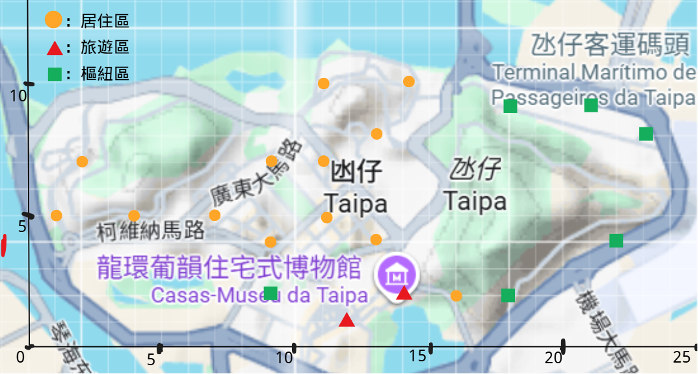
\includegraphics[width = \textwidth]{sections/images/投放.png}
    \caption{21處站點已標出的嘉模堂區地圖}
    \label{fig:cluster4_20}
\end{figure}
每個站點的初始投放量如下表所示.
\begin{table}[H]
    \begin{center}
        \begin{tabular}{ccccc}
        \hline
        站點編號 & 區域 & 對應坐標 & 實際地界 & 初始投放數量 \\
        \hline
        1 & 居住區 & (1,5) & 氹仔海洋花園衛生中心入口 & 5 \\
        2 & 居住區 & (2,7) & 海洋廣場入口 & 12 \\
        3 & 居住區 & (4,5) & 盈翠山莊馬路對面 & 8 \\
        4 & 居住區 & (7,5) & 澳門賽馬會賽事大樓入口左側 & 12 \\
        5 & 居住區 & (9,4) & 美景花園入口 & 15 \\
        6 & 居住區 & (9,7) & 鴻發花園入口右側 & 10 \\
        7 & 居住區 & (11,5) & 澳門大學附屬應用學校入口馬路對面 & 15 \\
        8 & 居住區 & (11,7) & 雄景花園入口 & 13 \\
        9 & 居住區 & (11,10) & 中福花園（麗怡閣）入口 & 10 \\
        10 & 居住區 & (13,4) & 泉悅花園入口 & 15 \\
        \vdots & \vdots & \vdots & \vdots & \vdots \\
        20 & 旅遊區 & (12,1) & 官也街 & 8 \\
        21 & 旅遊區 & (14,2) & 龍環葡韻 & 5 \\
        \hline
        \end{tabular}
    \end{center}
    \caption{共享單車站點的投放信息, {\color{red} \Large 附錄}}
\end{table}

\subsection{共享單車再平衡問題}
\subsubsection{目標函數}
為滿足用戶租還車需求, 運營商需要派遣調度卡車將共享單車從取貨點(初始庫存大於期望需求), 調送至送貨點(初始庫存小於期望需求), 以實現供求失衡站點的再平衡. 調度卡車從車場出發, 服務完一系列站點之後返回車場, 產生與之對應的運輸成本. 考慮到實際中卡車調度作業會受各種因素的限制(如預算限製與工作時長等), 為提高調度的靈活度, 本問題允許調度結果不滿足實際需求.即卡車可以在送貨點留下的單車數量小於期望需求, 或者在取貨點留下的單車數量大於期望需求. 然而若調度結果不滿足用戶需求, 會給用戶帶來不便, 因此我們需要一個與期望需求偏離時產生的懲罰成本\(p\).

本模型將該實際問題定義在有向圖\(G=(S_0, E)\)上. 其中站點集合\(S = P\cup D\)為取貨站點集合與卸貨站點集合的並集, \(S_0 = S\cup\{0\}\)為所有站點再額外加上車場\(0\). 邊集合\(E\)為所有站點之間的道路連接\(e\)(每條弧關聯運輸成本與運輸時間), 本問題需要確定卡車為哪些卡車提供服務、選擇哪些邊作為運輸路線以及在每一個站點的取貨與卸貨數量, 從而最小化總成本, 即為總運輸成本與懲罰成本之和.

該模型的目標函數為:
\begin{equation}
\min \sum_{i,j\in S_0}c_{ij}x_{ij} + \sum_{i\in S}\frac{p_i|s_i - s_i^I|}{s_i^I}
\end{equation}
其中\(c_{ij}\)為從站點\(i\)到站點\(j\)的運輸成本. 現實中\(c\)與路況、油耗以及員工薪水有關, 但為了簡化模型, 這裡認為\(c\)與運輸路程成正比例關係, 也就是認為\(c=k_c d(e_{ij})\), 其中\(d(e_{ij})\)為從站點\(i\)到站點\(j\)的道路長度.
\(x_{ij}\)為0-1變量, 表示是否選擇從站點\(i\)到站點\(j\)的邊.
\(p_i\)為站點\(i\)調度結束後庫存\(s_i(= s_i^0 - y_i)\)偏離期望需求\(s_i^I\)的懲罰成本. 
\subsubsection{庫存量約束}


調度貨車在每個站點的取貨數量\(y_i\)不能超過站點的初始庫存\(s_i^0\), 卸貨數量不能超過站點剩餘庫存\(l_i - s_i^0\),其中\(l_i\)為站點\(i\)的最大庫存. \(\sum_{j\in S_0}x_{ij}\)表示該站點是否被訪問, 如果被訪問則為1, 沒有被訪問則為0, 這樣就可以確保若該站點未被訪問, 則取貨數量與卸貨數量均為0.
\begin{gather}
y_i \leqslant s_i^0 \sum_{j\in S_0}x_{ij}, \forall i\in P\\
-y_i \leqslant \left(l_i - s_i^0\right)\sum_{j\in S_0}x_{ij}, \forall i\in D
\end{gather}
\subsubsection{流量約束}
根據{\color{red}\Large 假設}, 該模型不允許一輛卡車同時訪問一個站點多次, 因此對於每個站點\(i\), 其被訪問的邊\(x_{ij}\)的總和\(\sum x_{ij}\)需要小於等於1. 同時, 車場\(0\)需要被訪問一次, 而且卡車在最後必須回到車場, 於是得到以下兩個約束條件.
\begin{gather}
\sum_{j\in S_0}x_{ij} = \sum_{j\in S_0}x_{ji} \leqslant 1, \forall i\in S_0\\%每個站點只能被訪問一次
\sum_{j\in S_0}x_{0j} = \sum_{j\in S_0}x_{j0} = 1
\end{gather}
\subsubsection{貨車運載量約束}
接下來對貨車的運載量進行約束.若在出發時車場的庫存為\(g\), 則在出發時取貨量\(y_0\)以及貨車運載量\(Q_0\)為\(g\). 在每個站點進行裝貨以及卸貨操作後, 貨車的庫存量\(Q\)需要滿足以下約束條件. 若從站點\(i\)到站點\(j\)的邊被選擇, 則站點\(j\)的庫存量\(Q_j\)需要大於等於站點\(i\)的庫存量\(Q_i\)加上在i站點的取貨量(或卸貨量)\(y_i\). 當\(x_{ij} = 0\)時, 取一個充分大的常數\(M\), 即\(M(1-x_{ij})\)充分大, 使得\(Q_i + y_i -M(1-x_{ij})<0\), 令到該對\(Q\)的約束條件無效. 同時, 貨車在每個站點的運載量不能超過貨車的最大運載量\(C\). 相似地, 若該站點未被訪問, 則運載量為0.
\begin{gather}
Q_0 = y_0 =g \leqslant C\\
Q_j \geqslant Q_i + y_i - M(1-x_{ij}), \forall i,j\in S_0, i\neq j\\
Q_i \leqslant C\sum_{j\in S_0}x_{ij}, \forall i\in S_0
\end{gather}
\subsubsection{工作時間約束}
在運載過程中, 貨車的行駛時間不能超過預定的工作時間\(T_{工作}\). 記從站點\(i\)到站點\(j\)的行駛時間為\(t_{ij}\), 則在每個站點的行駛時間需要滿足以下約束條件. 規定從車場出發時的累計工作時間\(T_{累積}\) 為0. 在被訪問過的某個站點\(j\)上, 累計工作時間\({T_{累積}}_j \)需要大於等於從站點\(i\)到站點\(j\)的行駛時間\(t_{ij}\)加上在站點\(j\)的卸貨時間\(u_j\), 再加上在\(i\)點的累計工作時間\({T_{累積}}_i\). 而當\(j\)點未被訪問過時, 約束條件無效. 若貨車從\(i\)點返回車場, 則在\(i\)點的累計工作時間\({T_{累積}}_i \)加上從\(i\)點到車場的行駛時間\(t_{i0}\)需要小於等於預定的工作時間\(T_{工作}\).
\begin{gather}
{T_\text{累積}}_0 = 0\\
{T_\text{累積}}_j \geqslant {T_\text{累積}}_i + t_{ij} + u_j -  M(1-x_{ij}), \forall i\in S_0,j\in S, i\neq j\\
{T_\text{累積}}_i + t_{i0}(1-x_{i0}) \leqslant T,\forall i\in S
\end{gather}
在這裡, 根據{\color{red}\Large 假設}有每個站點的裝卸時間\(u_i \propto |y_i|\).

\subsubsection{多輛卡車調度模型}
該調度方案僅考慮了一台貨車的調度, 但實際中可能有多台貨車參與調度. 若該系統存在\(K\)輛調度卡車, 記為卡車集\(\mathcal{K}=\{1,2,\dots,K\}\). 每輛卡車有不同的運載量\(C^k\)與初始庫存\(g^k\), 並且每輛卡車的工作時間\(T^k\)也可能不同.在這種情況下, 我們需要對每輛卡車的調度進行建模. 對於每輛卡車\(k\), 我們可以定義一個與上述單輛卡車調度模型類似的目標函數:
\begin{equation}
\min \sum_{k\in \mathcal{K}}\sum_{i,j\in S_0}c_{ij}x_{ij}^k + \sum_{i\in S}p_i|s_i - s_i^{I}|
\end{equation}
其中\(x_{ij}^k\)表示卡車\(k\)是否選擇從站點\(i\)到站點\(j\)的邊, \(s_i^k\)為卡車\(k\)在站點\(i\)的庫存量, \(s_i^{I,k}\)為卡車\(k\)在站點\(i\)的期望需求. 
對於每輛卡車\(k\), 由於前文的所有約束條件均與卡車的整體調度方案無關, 因此我們可以將上述約束條件套用到每輛卡車上, 即為原有約束條件添加上標\(k\). 另外, 卡車\(k\)從倉庫出發時的庫存量\(g^k\)之和不能超過倉庫的總車輛, 但根據{\color{red}\Large 假設[]}, 倉庫有充分多的共享單車, 不會被卡車用盡. 

另外, 為了確保站點不會被不同卡車訪問多次, 我們需要對每個站點的訪問進行約束. 具體來說, 對於每個站點\(i\), 所有卡車\(k\)的訪問邊\(x_{ij}^k\)的總和需要小於等於1, 即
\begin{equation}
\sum_{k\in \mathcal{K}}\sum_{j\in S_0}x_{ij}^k \leqslant 1, \forall i\in S_0
\end{equation}

這樣就得到了多輛卡車調度模型的完整描述.

\subsubsection{模型參數的選取}
根據前文, 站點可以被分為樞紐區\(S_T\)、居民區\(S_R\)以及旅遊區\(S_H\), 即\(S = S_T\cup S_R\cup S_H\). 因此, 對於\(S\)中的每一個站點可以選擇不同的懲罰成本\(p_i\in\{p_T, p_R, p_H\}\). 具體來說, 樞紐區的懲罰成本\(p_T\)可以設置為0, 因為這些站點的期望需求通常較高且穩定,
而居民區的懲罰成本\(p_R\)可以設置為較低的值, 因為這些站點的期望需求較低且波動較大, 最後旅遊區的懲罰成本\(p_H\)可以設置為較高的值, 因為這些站點的期望需求通常較高且波動較大. 這樣的設置可以使得調度方案更符合實際需求, 並且能夠更好地平衡各個站點的庫存與需求. 若在其他城市中有其他適用的分區方案, 可以套用本模型進行參數的選取.

每段道路的運輸成本\(c_{ij}\)可以根據實際情況進行設置, 例如可以考慮道路的長度、交通狀況等因素. 對於每輛卡車的運載量\(C^k\)與初始庫存\(g^k\), 可以根據實際情況進行設置,例如可以考慮卡車的大小、載重能力等因素. 道路的長度\(d(e)\)可以通過市面上的導航係統獲取(如高德地圖、百度地圖等), 而道路的交通狀況可以通過實時交通數據獲取(如高德地圖的實時路況數據).
對於每個站點的裝卸時間\(u_i\), 可以根據實際情況進行設置, 例如可以考慮站點員工的工作效率. 同樣地,每位員工的工作時間\(T_\text{工作}^k\)也可以根據實際情況進行設置. 這些參數的選取可以根據實際情況進行調整, 以使得調度方案更符合實際需求.

\subsubsection{模型求解與調度信息}
考慮到在實際中搜集\(N\)個站點兩兩之間的距離將產生\(N(N-1)\)條有向邊, 因此該模型的計算量較大. 因此, 在此模型中, 我們將使用兩點之間的曼哈頓距離, 即對於點\(\mathbf{x}\)和\(\mathbf{y}\), 其曼哈頓距離為
\begin{equation}
d(\mathbf{x}, \mathbf{y}) = |x_1 - y_1| + |x_2 - y_2|
\end{equation}
這樣可以大大減少計算量, 並且在實際中也能夠較好地反映兩點之間的距離.
另外, 由於用戶的騎車行為難以預測, 並且在澳門未有足夠的歷史數據進行訓練, 因此我們將利用幾組隨機數作為原投放量, 將前文的初始投放數量作為目標投放量進行優化.
對於其他的參數, 我們將根據前文的討論進行設置. 
\begin{enumerate}
    \item 最大庫存設置為\(l_i=\left\lceil 150\% s_i^I  \right\rceil\).
    為了確保每個站點歸還單車時有樁可用, 我們將站點的最大庫存設置為期望需求的150\%, 這樣可以確保在還車時有充分的餘量.
    \item 根据《道路旅客運輸企業安全管理規範》相關要求, 貨車的最大工作時間\(T_\text{工作}= 120 \text{min}\).
    \item 貨車的最大運載量\(C= 40\), 這是根據澳門的道路狀況以及貨車的實際情況進行設置的. 澳門道路狹窄, 貨車的運載量需要控制在一定範圍內, 以確保道路安全.
    \item 根據不同地區(居住區、旅遊區、樞紐區)的需求特點, 我們將懲罰成本設置為
    \begin{itemize}
        \item 居民區\(p_T=200\), 因為這些站點的期望需求通常較高且穩定, 不需要懲罰成本;
        \item 樞紐區\(p_R=400\), 因為這些站點的期望需求較低且波動較大, 需要一定的懲罰成本來平衡庫存與需求;
        \item 旅遊區\(p_H=600\), 因為這些站點的期望需求通常較高且波動較大, 需要較高的懲罰成本來平衡庫存與需求.
    \end{itemize}
    並且, 通過數值試驗, 該參數與距離的數量級相當, 這樣可以確保懲罰成本在目標函數中有足夠的影響力.
    \item 裝卸時間係數設置為\(k_u = 0.2 \text{min/車}\). 這是根據實際情況決定的.
    \item 運輸成本設置為\(c_{ij} = d(e_{ij})\). 
    \item 根據{\color{red} \Large 假設}, 車輛到達下一個站點的時間正比於站點之間的距離, 即\(t_{ij} = k_td(e_{ij})\). 在這裡將\(k_t\)設置為\(0.00167\text{min/km}\), 約每小時40公里的速度.
\end{enumerate}
將參數輸入到{\color{red}\Large 附錄}的程序中, 測試用例(即每個站點的自行車數量)如{\color{red} \Large 附錄[]所示}, 運行得到以下結果. 
\begin{table}[H]
    \begin{center}
        \begin{tabular}{cccccccccc}
            \hline
            站点  & 区域 & 操作量 & 初始库存 & 最终库存 & 期望库存 & 库存偏差 & 是否访问 & 惩罚成本 \\
            \hline
            4  & 居住區 & 4.0 & 16 & 12.0 & 12 & 0.0 & 是 & 0.0 \\
            5  & 居住區 & 5.0 & 20 & 15.0 & 15 & 0.0 & 是 & 0.0 \\
            14  & 樞紐區 & 1.0 & 26 & 25.0 & 25 & 0.0 & 是 & 0.0 \\
            19  & 樞紐區 & -20.0 & 10 & 30.0 & 30 & 0.0 & 是 & 0.0 \\
            2  & 居住區 & -12.0 & 0 & 12.0 & 12 & 0.0 & 是 & 0.0 \\
            18  & 樞紐區 & -5.0 & 20 & 25.0 & 25 & 0.0 & 是 & 0.0 \\
            9  & 居住區 & 0.0 & 9 & 9.0 & 10 & 1.0 & 否 & 1000.0 \\
            11  & 居住區 & 0.0 & 5 & 5.0 & 8 & 3.0 & 否 & 3000.0 \\
            12  & 居住區 & 0.0 & 3 & 3.0 & 10 & 7.0 & 否 & 7000.0 \\
            15  & 樞紐區 & 0.0 & 13 & 13.0 & 14 & 1.0 & 否 & 2000.0 \\
            21  & 旅遊區 & 0.0 & 7 & 7.0 & 5 & 2.0 & 否 & 6000.0 \\
            \hline
        \end{tabular}
    \end{center}
    \caption{調度完成後的站點信息}
\end{table}
\begin{table}[H]
    \begin{center}
        \begin{tabular}{cccccc}
            \hline
            从站点 & 到站点 & 距离(米) & 操作量 & 操作时间 & 累计时间(分) \\
            \hline
            0 & 14 & 4200.0 & 0.0 & 0.00 & 7.01 \\
            14 & 5 & 900.0 & 1.0 & 0.20 & 8.71 \\
            5 & 4 & 450.0 & 5.0 & 1.00 & 10.46 \\
            4 & 13 & 2250.0 & 4.0 & 0.80 & 14.61 \\
            13 & 19 & 1200.0 & 0.0 & 0.00 & 16.61 \\
            19 & 18 & 1200.0 & -20.0 & 4.00 & 22.61 \\
            18 & 2 & 31500.0 & -5.0 & 1.00 & 76.11 \\
            2 & 0 & 34500.0 & -12.0 & 2.40 & 115.51 \\
            \hline
        \end{tabular}
    \end{center}
    \caption{貨車調度路線以及在該站點的裝卸信息}
\end{table}

在該調度方式下, 總成本為34000(無量綱), 其中運輸成本為15500, 懲罰成本為19000.

在這裡由於約束條件較緊, 卡車無法再固定的容量和時間內滿足所有站點的需求, 例如站點9的期望需求為\(s_i^I=10\), 但調度結果為\(s_i=9\)(未訪問), 即該站點的庫存量小於期望需求, 
因此產生了懲罰成本. 但這已經是在該約束條件下令目標函數最小化的結果, 若需要滿足這些站點的全部需求, 我們需要放寬約束條件或者調度另一輛卡車同時進行共享單車的調度作業.
\newpage

\section{靈敏度分析}
\input{sections/sensitivity.tex}
\newpage

\section{模型優劣分析}
\subsection{優勢}
\begin{enumerate}
    \item \textbf{精細區域劃分}：根據氹仔的地理與功能特徵，將區域分為居民區、旅遊區和樞紐區，針對性地優化站點與投放量，提升了模型的適用性。
    \item \textbf{多因素綜合考慮}：模型整合了空間異質性、時間不對稱性和資源限制等多維約束，使優化結果更貼近實際需求。
    \item \textbf{靈活再平衡策略}：通過引入懲罰成本，允許不完全滿足需求，平衡了運輸成本與用戶體驗，提升了運營靈活性。
    \item \textbf{可擴展性}：支持多輛卡車調度，適應不同規模的運營需求，具有較好的擴展潛力。
\end{enumerate}

\subsection{劣勢}
\begin{enumerate}
    \item \textbf{數據依賴性}：模型效果依賴於歷史需求的準確性，若數據質量不足，優化結果可能失真。
    \item \textbf{計算複雜度}：隨著站點數增加，混合整數規劃與調度模型的求解難度上升，可能需要更高效的算法。
    \item \textbf{參數調節挑戰}：懲罰成本與運輸成本係數等參數需根據實際情況精確設置，否則可能影響結果。
    \item \textbf{動態性不足}：模型以靜態優化為主，對實時需求變化的響應能力有限。
\end{enumerate}

\newpage

\section{總結}
本研究開發了一個針對澳門氹仔地區共享單車系統的綜合優化框架，涵蓋站點選址、初始投放量優化和再平衡問題。在選址與投放方面，模型通過將區域細分為居民區、旅遊區和樞紐區，並基於歷史需求數據估計淨需求流量，採用混合整數規劃方法確定最佳站點位置與初始投放量，以最小化高峰時段的服務缺口。結果顯示，21個站點和280輛單車的配置下，全局最大服務缺口為12，總缺口為65，滿足了空間容量與預算約束。在再平衡方面，模型構建了一個基於有向圖的調度方案，考慮運輸成本、懲罰成本及卡車運載量等實際約束，允許不完全滿足需求以提升靈活性，並支持多輛卡車調度。通過數值試驗，該模型在單車調度中實現了總成本的最優化（運輸成本15500，懲罰成本19000），為運營決策提供了參考。整體而言，該模型結合理論與實踐，為共享單車系統的高效運行提供了科學工具。

% \section{參考文獻}
% \begin{enumerate}[ {[}1{]} ]
%   \item FootballDatabase.com. (n.d.). FootballDatabase - Club rankings and statistics. FootballDatabase. https://footballdatabase.com/\#google\_vignette
%   \item Miratrix, L. W., Sekhon, J. S., Theodoridis, A. G., \& Campos, L. F. (2018). Worth Weighting? How to think about and use weights in survey experiments. Political Analysis, 26(3), 275–291. https://doi.org/10.1017/pan.2018.1
%   \item NBA Team standings \& Stats | NBA.com. (n.d.). NBA. https://www.nba.com/standings
%   \item NBA.com Staff. (2024, September 24). All 30 NBA arenas by team. NBA. \\https://www.nba.com/news/all-30-nba-arenas-by-team
%   \item Ritchie, C., \& Hepburn, D. (2025, January 11). Ranking the 25 best stadiums in world football (2025). GiveMeSport. https://www.givemesport.com/best-football-soccer-stadiums-ranked/
%   \item Saaty, T. L., \& Vargas, L. G. (2012). Models, Methods, Concepts \& Applications of the Analytic Hierarchy Process. In International series in management science/operations research/International series in operations research \& management science. https://doi.org/10.1007/978-1-4614-3597-6
%   \item Wang, Z. (2023). Research on the Strategy of Holding Olympic Games based on AHP and FCE. Highlights in Science Engineering and Technology, 49, 130–135. \\https://doi.org/10.54097/hset.v49i.8491
% \end{enumerate}

\newpage

\begin{appendices}
  \section{圖表}
  \label{appendix:graph}
  \begin{table}[H]
    \begin{center}
        \begin{tabular}{ccccc}
        \hline
        站點編號 & 區域 & 對應坐標 & 實際地界 & 初始投放數量 \\
        \hline
        1 & 居住區 & (1,5) & 氹仔海洋花園衛生中心入口 & 5 \\
        2 & 居住區 & (2,7) & 海洋廣場入口 & 12 \\
        3 & 居住區 & (4,5) & 盈翠山莊馬路對面 & 8 \\
        4 & 居住區 & (7,5) & 澳門賽馬會賽事大樓入口左側 & 12 \\
        5 & 居住區 & (9,4) & 美景花園入口 & 15 \\
        6 & 居住區 & (9,7) & 鴻發花園入口右側 & 10 \\
        7 & 居住區 & (11,5) & 澳門大學附屬應用學校入口馬路對面 & 15 \\
        8 & 居住區 & (11,7) & 雄景花園入口 & 13 \\
        9 & 居住區 & (11,10) & 中福花園（麗怡閣）入口 & 10 \\
        10 & 居住區 & (13,4) & 泉悅花園入口 & 15 \\
        11 & 居住區 & (13,8) & 仁伯爵綜合醫院精神科大樓入口右側 & 8 \\
        12 & 居住區 & (14,10) & 海明灣畔入口 & 10 \\
        13 & 居住區 & (16,2) & 大潭山壹號入口 & 10 \\
        14 & 樞紐區 & (9,2) & 澳門運動場 & 25 \\
        15 & 樞紐區 & (18,9) & 新南工業大廈入口 & 14 \\
        16 & 樞紐區 & (21,9) & 新城混凝土廠入口 & 18 \\
        17 & 樞紐區 & (23,8) & 南光北安油站左側 & 17 \\
        18 & 樞紐區 & (22,4) & 澳門國際機場客運大樓出口前方 & 25 \\
        19 & 樞紐區 & (18,2) & 澳門科技大學入口 & 30 \\
        20 & 旅遊區 & (12,1) & 官也街 & 8 \\
        21 & 旅遊區 & (14,2) & 龍環葡韻 & 5 \\
        \hline
        \end{tabular}
    \end{center}
    \caption{21處站點的信息}
\end{table}
\begin{table}[H]
    \begin{center}
        \begin{tabular}{ccccc}
            \hline
            站點 & 類型 & 裝/卸量(\(y_i\)) & 庫存偏差 & 卡車裝載量(\(Q_i\))\\
            \hline
            0 & 車場 & 108 & / & 0\\
            18 & 卸貨站點 & -10 & 0 & 108\\
            17 & 卸貨站點 & -7 & 0 & 98\\
            16 & 卸貨站點 & -7 & 0 & 91\\
            15 & 卸貨站點 & -6 & 0 & 84\\
            12 & 卸貨站點 & -4 & 0 & 78\\
            9 & 卸貨站點 & -4 & 0 & 74\\
            11 & 卸貨站點 & -3 & 0 & 70\\
            10 & 卸貨站點 & -6 & 0 & 67\\
            7 & 卸貨站點 & -6 & 0 & 61\\
            8 & 卸貨站點 & -5 & 0 & 55\\
            6 & 卸貨站點 & -4 & 0 & 50\\
            2 & 卸貨站點 & -2 & 0 & 46\\
            1 & 卸貨站點 & -2 & 0 & 44\\
            3 & 卸貨站點 & -3 & 0 & 42\\
            4 & 卸貨站點 & -2 & 0 & 39\\
            5 & 卸貨站點 & -6 & 0 & 37\\
            14 & 卸貨站點 & -10 & 0 & 31\\
            20 & 卸貨站點 & -3 & 0 & 21\\
            21 & 卸貨站點 & -2 & 0 & 18\\
            13 & 卸貨站點 & -4 & 0 & 16\\
            19 & 卸貨站點 & -12 & 0 & 12\\
            0 & 車場 & 0 & / & 0\\
        \hline
        \end{tabular}
    \end{center}
    \caption{21處站點的信息}
\end{table}

\newpage
  \section{代碼}
  \subsection{共享單車投放及選址代碼}
  \begin{minted}{python3}
import gurobipy as gp
from gurobipy import GRB

class BikeAllocationSolver:
    def __init__(self, S, S_R, S_T, S_H, R, N, c, f, B, N_max, gamma, q):
        self.data = {
            'S': S, 'S_R': S_R, 'S_T': S_T, 'S_H': S_H,
            'R': R, 'N': N, 'c': c, 'f': f,
            'B': B, 'N_max': N_max, 'gamma': gamma, 'q': q
        }
        self.model = gp.Model("Bike_Allocation_Core")
        self.results = {}
    
    def solve(self):
        """執行模型求解全過程"""
        self._init_variables()
        self._add_constraints()
        self._set_objective()
        self._optimize()
        return self._extract_solution()

    def _init_variables(self):
        """初始化決策變數"""
        d = self.data
        
        # 選址決策 (二進位)
        self.Y = self.model.addVars(d['S'], vtype=GRB.BINARY, name="Y")
        
        # 投放量決策 (整數)
        self.X = self.model.addVars(d['S'], vtype=GRB.INTEGER, lb=0, name="X")
        
        # 服務缺口變數
        self.alpha = self.model.addVars(d['S'], vtype=GRB.CONTINUOUS, lb=0, name="alpha")
        self.beta = self.model.addVars(d['S'], vtype=GRB.CONTINUOUS, lb=0, name="beta")
        
        # 全域缺口目標
        self.Phi_max = self.model.addVar(vtype=GRB.CONTINUOUS, lb=0, name="Phi_max")
        self.Phi_sum = self.model.addVar(vtype=GRB.CONTINUOUS, lb=0, name="Phi_sum")

    def _add_constraints(self):
        """構建模型約束系統"""
        d = self.data
        
        # 約束1: 容量約束 (0 ≤ Xₛ ≤ cₛYₛ)
        self.model.addConstrs(self.X[s] <= d['c'][s] * self.Y[s] for s in d['S'])
        self.model.addConstrs(self.X[s] >= 0 for s in d['S'])
        
        # 約束2: 總量約束 (∑Xₛ ≤ B)
        self.model.addConstr(gp.quicksum(self.X[s] for s in d['S']) <= d['B'])
        
        # 約束3: 站點數約束 (∑Yₛ ≤ N_max)
        self.model.addConstr(gp.quicksum(self.Y[s] for s in d['S']) <= d['N_max'])
        
        # 約束4: 即時庫存計算
        G = {}
        for s in d['S']:
            G[s] = [self.X[s]]  # τ=0
            for m in range(1, d['q']+1):
                cum_flow = gp.quicksum(d['f'][s][i] for i in range(m))
                G[s].append(self.X[s] + cum_flow)
        
        # 約束5: 借車缺口定義 (α_s)
        for s in d['S']:
            # α_s ≥ -G_m^s (∀m)
            self.model.addConstrs(self.alpha[s] >= -G[s][m] for m in range(1, d['q']+1))
            self.model.addConstr(self.alpha[s] >= 0)
        
        # 約束6: 還車缺口定義 (β_s)
        for s in d['S']:
            # β_s ≥ G_m^s - c_s (∀m)
            self.model.addConstrs(self.beta[s] >= G[s][m] - d['c'][s] for m in range(1, d['q']+1))
            self.model.addConstr(self.beta[s] >= 0)
        
        # 約束7: 全域最大缺口 (Φ_max)
        for s in d['S']:
            self.model.addConstr(self.Phi_max >= self.alpha[s])
            self.model.addConstr(self.Phi_max >= self.beta[s])
        
        # 約束8: 缺口總和 (Φ_sum)
        self.model.addConstr(
            self.Phi_sum == gp.quicksum(
                (self.alpha[s] + self.beta[s]) * self.Y[s] for s in d['S']
            )
        )
        
        # 約束9: 功能區最小站點數
        self.model.addConstr(
            gp.quicksum(self.Y[s] for s in d['S_R']) >= d['gamma']['R']
        )
        self.model.addConstr(
            gp.quicksum(self.Y[s] for s in d['S_T']) >= d['gamma']['T']
        )
        self.model.addConstr(
            gp.quicksum(self.Y[s] for s in d['S_H']) >= d['gamma']['H']
        )
        
        # 約束10: 居民點可達性
        for r in d['R']:
            self.model.addConstr(
                gp.quicksum(self.Y[s] for s in d['N'][r]) >= 1
            )

    def _set_objective(self):
        """設置目標函數 (λ=0.8)"""
        self.model.setObjective(
            0.8 * self.Phi_max + 0.2 * self.Phi_sum,
            GRB.MINIMIZE
        )

    def _optimize(self):
        """執行優化計算"""
        self.model.setParam('OutputFlag', 0)  # 關閉求解日誌
        self.model.optimize()

    def _extract_solution(self):
        """提取優化結果"""
        if self.model.status == GRB.OPTIMAL:
            return {
                'status': 'OPTIMAL',
                'Y': {s: self.Y[s].X for s in self.data['S']},
                'X': {s: self.X[s].X for s in self.data['S']},
                'alpha': {s: self.alpha[s].X for s in self.data['S']},
                'beta': {s: self.beta[s].X for s in self.data['S']},
                'Phi_max': self.Phi_max.X,
                'Phi_sum': self.Phi_sum.X,
                'obj_value': self.model.ObjVal
            }
        else:
            return {'status': self.model.status}
\end{minted}
  \subsection{共享單車再平衡代碼}
  \begin{minted}{python3}
import pulp
import numpy as np
import math
import time

# =============================
# 參數設定 (基於提供的數據)
# 站點座標
coordinates = {
    0: (25, -5),   # 車場
    1: (1, 5),    2: (2, 7),     3: (4, 5),     4: (7, 5),
    5: (9, 4),    6: (9, 7),     7: (11, 5),    8: (11, 7),
    9: (11, 10),  10: (13, 4),   11: (13, 8),   12: (14, 10),
    13: (16, 2),  14: (9, 2),    15: (18, 9),   16: (21, 9),
    17: (23, 8),  18: (22, 4),   19: (18, 2),   20: (12, 1),
    21: (14, 2)
}

# 站點類型
site_types = {
    1: "居住區", 2: "居住區", 3: "居住區", 4: "居住區", 5: "居住區",
    6: "居住區", 7: "居住區", 8: "居住區", 9: "居住區", 10: "居住區",
    11: "居住區", 12: "居住區", 13: "居住區", 14: "樞紐區", 15: "樞紐區",
    16: "樞紐區", 17: "樞紐區", 18: "樞紐區", 19: "樞紐區", 20: "旅遊區",
    21: "旅遊區"
}

# 期望庫存 sI
sI = {
    0: 0, 1: 5, 2: 12, 3: 8, 4: 12,
    5: 15, 6: 10, 7: 15, 8: 13, 9: 10,
    10: 15, 11: 8, 12: 10, 13: 10, 14: 25,
    15: 14, 16: 18, 17: 17, 18: 25, 19: 30,
    20: 8, 21: 5
}

# 初始庫存 s0
s0 = {
    0: 0, 1: 5, 2: 0, 3: 8, 4: 16,
    5: 20, 6: 10, 7: 15, 8: 14, 9: 9,
    10: 16, 11: 5, 12: 3, 13: 14, 14: 26,
    15: 13, 16: 18, 17: 17, 18: 20, 19: 10,
    20: 8, 21: 7
}

# 計算最大庫存 l = sI * 1.5 向上取整
l = {i: math.ceil(sI[i] * 1.5) for i in range(22)}

# 懲罰係數 p
p_cost = {0: 0}
for i in range(1, 22):
    if site_types[i] == "居住區":
        p_cost[i] = 1000
    elif site_types[i] == "樞紐區":
        p_cost[i] = 2000
    else:  # 旅遊區
        p_cost[i] = 3000

# 卡車參數
C = 40          # 卡車容量
T_work = 120    # 最大工作時間 (分鐘)
alpha = 0.2     # 裝卸時間係數 (分鐘/單車)

# 計算曼哈頓距離
def manhattan_distance(coord1, coord2):
    return 150 * (abs(coord1[0] - coord2[0]) + abs(coord1[1] - coord2[1]))

# 創建距離矩陣
distances = {}
for i in range(22):
    for j in range(22):
        if i == j:
            distances[(i, j)] = 0
        else:
            distances[(i, j)] = manhattan_distance(coordinates[i], coordinates[j])

# 時間矩陣 = 距離矩陣 * 0.00167
times = {key: value * 0.00167 for key, value in distances.items()}

# 大M常數
M = 100000

# 站點集合
S0 = list(range(22))  # 所有站點，包括車場
P = [i for i in range(1, 22) if s0[i] > sI[i]]  # 取貨站 (初始庫存 > 期望庫存)
D = [i for i in range(1, 22) if s0[i] < sI[i]]  # 送貨站 (初始庫存 < 期望庫存)
S = P + D  # 需要服務的站點

# 列印參數概覽
print("站點類型分布:")
print(f"車場: 0")
print(f"取貨站 ({len(P)}個): {P}")
print(f"送貨站 ({len(D)}個): {D}")
print(f"平衡站 ({22 - len(S) - 1}個): {set(range(1, 22)) - set(P) - set(D)}")

print("\n關鍵參數示例:")
print(f"站點4 (取貨站): 初始庫存={s0[4]}, 期望庫存={sI[4]}, 最大庫存={l[4]}, 懲罰係數={p_cost[4]}")
print(f"站點2 (送貨站): 初始庫存={s0[2]}, 期望庫存={sI[2]}, 最大庫存={l[2]}, 懲罰係數={p_cost[2]}")
print(f"站點19 (樞紐區送貨站): 初始庫存={s0[19]}, 期望庫存={sI[19]}, 最大庫存={l[19]}, 懲罰係數={p_cost[19]}")
print(f"站點21 (旅遊區取貨站): 初始庫存={s0[21]}, 期望庫存={sI[21]}, 最大庫存={l[21]}, 懲罰係數={p_cost[21]}")

print(f"\n卡車參數: 容量={C}, 最大工作時間={T_work}分鐘")
print(f"裝卸時間係數: {alpha} 分鐘/單車")

# =============================
# 創建優化模型
# =============================
model = pulp.LpProblem("Bike_Sharing_Scheduling", pulp.LpMinimize)

# =============================
# 定義決策變數
# =============================
# 路徑變數 x_ij
x = pulp.LpVariable.dicts("x", ((i, j) for i in S0 for j in S0 if i != j), 
                          cat=pulp.LpBinary)

# 站點操作量 y_i
y = pulp.LpVariable.dicts("y", S0, lowBound=-C, upBound=C, cat=pulp.LpContinuous)

# 卡車裝載量 (到達站點i時的裝載量)
Q_arrive = pulp.LpVariable.dicts("Q_arrive", S0, lowBound=0, upBound=C, cat=pulp.LpContinuous)

# 累計時間 (離開站點i時的時間)
T_leave = pulp.LpVariable.dicts("T_leave", S0, lowBound=0, upBound=T_work, cat=pulp.LpContinuous)

# 庫存偏差 delta_i = |s_i - sI_i|
delta = pulp.LpVariable.dicts("delta", S0, lowBound=0, cat=pulp.LpContinuous)

# 輔助變數: 站點是否被訪問
visited = pulp.LpVariable.dicts("visited", S, cat=pulp.LpBinary)

# =============================
# 目標函數：運輸成本 + 懲罰成本
# =============================
# 運輸成本使用距離（而不是時間）計算
transport_cost = pulp.lpSum(distances[(i, j)] * x[i, j] for i in S0 for j in S0 if i != j)
penalty_cost = pulp.lpSum(p_cost[i] * delta[i] for i in S)
model += transport_cost + penalty_cost

# =============================
# 約束條件
# =============================
# 1. 車場訪問約束 - 必須從車場出發並返回
model += pulp.lpSum(x[0, j] for j in S) == 1  # 從車場出發
model += pulp.lpSum(x[i, 0] for i in S) == 1  # 返回車場

# 2. 站點訪問約束
for i in S:
    # 入度 = 出度
    model += pulp.lpSum(x[i, j] for j in S0 if j != i) == pulp.lpSum(x[j, i] for j in S0 if j != i)
    
    # 訪問標記約束
    model += visited[i] == pulp.lpSum(x[i, j] for j in S0 if j != i)

# 3. 車場特殊約束
model += y[0] == 0  # 車場無操作
model += Q_arrive[0] == 0  # 車場到達時裝載量為0
model += T_leave[0] == 0  # 車場離開時間為0

# 4. 庫存操作約束
for i in P:
    # 取貨站: 0 ≤ y_i ≤ min(s0[i] - sI[i], C)
    max_take = min(s0[i] - sI[i], C)
    model += y[i] >= 0
    model += y[i] <= max_take * visited[i]
    
for i in D:
    # 送貨站: -min(sI[i] - s0[i], C) ≤ y_i ≤ 0
    max_deliver = min(sI[i] - s0[i], C)
    model += y[i] <= 0
    model += y[i] >= -max_deliver * visited[i]

# 5. 卡車裝載量約束
for i in S0:
    # 未訪問站點裝載量為0
    if i in S:
        model += Q_arrive[i] <= C * visited[i]
    else:
        model += Q_arrive[i] == 0
    
    # 離開裝載量 = 到達裝載量 + 操作量
    model += Q_arrive[i] + y[i] <= C  # 容量上限
    model += Q_arrive[i] + y[i] >= 0  # 非負
    
    # 裝載量連續性 (使用大M法)
    for k in S0:
        if k != i:
            model += Q_arrive[i] >= (Q_arrive[k] + y[k]) - M * (1 - x[k, i])
            model += Q_arrive[i] <= (Q_arrive[k] + y[k]) + M * (1 - x[k, i])

# 6. 時間約束
for i in S0:
    # 操作時間 = alpha * |y_i|
    # 線性化 |y_i|
    abs_y = pulp.LpVariable(f"abs_y_{i}", lowBound=0, upBound=C, cat=pulp.LpContinuous)
    model += abs_y >= y[i]
    model += abs_y >= -y[i]
    
    # 時間連續性
    for k in S0:
        if k != i:
            model += T_leave[i] >= T_leave[k] + times[(k, i)] + alpha * abs_y - M * (1 - x[k, i])
    
    # 返回車場時間約束
    if i != 0:
        model += T_leave[i] + times[(i, 0)] <= T_work + M * (1 - x[i, 0])

# 7. 庫存偏差約束
for i in S0:
    # 最終庫存 = 初始庫存 - 操作量
    # 偏差 = |最終庫存 - 期望庫存|
    model += delta[i] >= (s0[i] - y[i]) - sI[i]
    model += delta[i] >= sI[i] - (s0[i] - y[i])
    
    # 未訪問時偏差固定為|初始庫存 - 期望庫存|
    if i in S:
        model += delta[i] <= abs(s0[i] - sI[i]) + M * (1 - visited[i])
        model += delta[i] >= abs(s0[i] - sI[i]) - M * visited[i]

# =============================
# 求解模型
# =============================
start_time = time.time()
# 設定求解時間限制為300秒
model.solve(pulp.PULP_CBC_CMD(msg=True, timeLimit=300, gapRel=0.1))
solving_time = time.time() - start_time
status = pulp.LpStatus[model.status]
print(f"\n求解狀態: {status}")
print(f"求解時間: {solving_time:.2f}秒")

if status in ['Optimal', 'Feasible']:
    total_cost = pulp.value(model.objective)
    transport_cost_val = pulp.value(transport_cost)
    penalty_cost_val = pulp.value(penalty_cost)
    print(f"總成本: {total_cost:.2f}")
    print(f"運輸成本: {transport_cost_val:.2f}")
    print(f"懲罰成本: {penalty_cost_val:.2f}")
    print(f"懲罰成本占比: {100*penalty_cost_val/total_cost:.1f}%")
    
    # 計算訪問站點數量
    visited_count = sum(pulp.value(visited[i]) > 0.5 for i in S)
    print(f"訪問站點數: {visited_count}/{len(S)}")
else:
    print("未找到可行解，請嘗試放寬約束或增加資源")
    exit()

# =============================
# 結果解析與輸出
# =============================
def extract_route(x_vars, start=0):
    """提取卡車行駛路徑"""
    # 找到從車場出發的弧
    from_depot = [j for j in S0 if j != start and pulp.value(x_vars[start, j]) > 0.5]
    if not from_depot:
        return [start]
    
    route = [start]
    current = start
    next_node = from_depot[0]
    
    while next_node != start:
        route.append(next_node)
        # 找到下一個節點
        next_candidates = [j for j in S0 if j != next_node and pulp.value(x_vars[next_node, j]) > 0.5]
        
        if not next_candidates:
            break
            
        current = next_node
        next_node = next_candidates[0]
    
    # 返回車場
    if pulp.value(x_vars[route[-1], start]) > 0.5:
        route.append(start)
    
    return route

truck_route = extract_route(x)
print("\n卡車工作路線: " + " -> ".join(map(str, truck_route)))

# 計算總距離和總時間
total_distance = 0
total_time = 0
for i in range(len(truck_route)-1):
    from_node = truck_route[i]
    to_node = truck_route[i+1]
    total_distance += distances[(from_node, to_node)]
    
    # 在出發節點操作（除了車場）
    if from_node != 0:
        op = pulp.value(y[from_node])
        op_time = alpha * abs(op)
        total_time += op_time
    
    # 添加行駛時間
    travel_time = times[(from_node, to_node)]
    total_time += travel_time

print(f"總行駛距離: {total_distance:.2f} 米")
print(f"預估總時間: {total_time:.2f} 分鐘 (最大允許: {T_work}分鐘)")

# 輸出各站點操作詳情
print("\n各站點操作詳情:")
print("站點 | 類型   | 區域   | 操作量 | 初始庫存 | 最終庫存 | 期望庫存 | 庫存偏差 | 是否訪問 | 懲罰成本")
for i in range(1, 22):
    site_type = site_types[i]
    area = "居住區" if i <= 13 else ("樞紐區" if i <= 19 else "旅遊區")
    
    if i in S:
        is_visited = pulp.value(visited[i]) > 0.5
        op = pulp.value(y[i]) if is_visited else 0
    else:
        is_visited = False
        op = 0
    
    final_stock = s0[i] - op
    stock_dev = abs(final_stock - sI[i])
    penalty = p_cost[i] * stock_dev
    visit_flag = "✓" if is_visited else "✗"
    
    print(f"{i:3d} | {site_type:5s} | {area:5s} | {op:6.1f} | {s0[i]:8d} | {final_stock:8.1f} | {sI[i]:8d} | {stock_dev:7.1f} | {visit_flag:^7s} | {penalty:9.1f}")

# 輸出路徑詳情
print("\n路徑詳情:")
print("順序 | 從站點 | 到站點 |  距離(米) | 操作量 | 操作時間 | 累計時間(分)")
cumulative_time = 0
for idx in range(len(truck_route)-1):
    from_node = truck_route[idx]
    to_node = truck_route[idx+1]
    dist = distances[(from_node, to_node)]
    travel_time = times[(from_node, to_node)]
    
    # 在出發節點操作（除了車場）
    if from_node != 0:
        op = pulp.value(y[from_node])
        op_time = alpha * abs(op)
    else:
        op = 0
        op_time = 0
    
    cumulative_time += op_time + travel_time
    
    print(f"{idx+1:3d} | {from_node:5d} | {to_node:5d} | {dist:9.1f} | {op:6.1f} | {op_time:7.2f} | {cumulative_time:10.2f}")

# 最終返回車場
if truck_route[-1] == 0:
    print(f"卡車成功返回車場，總時間: {cumulative_time:.2f}分鐘")
else:
    print(f"注意: 卡車未返回車場! 最後位置: {truck_route[-1]}")

# 輸出未訪問站點
unvisited = [i for i in S if pulp.value(visited[i]) < 0.5]
if unvisited:
    print("\n未訪問站點:")
    total_penalty = 0
    for i in unvisited:
        site_type = site_types[i]
        area = "居住區" if i <= 13 else ("樞紐區" if i <= 19 else "旅遊區")
        stock_dev = abs(s0[i] - sI[i])
        penalty = p_cost[i] * stock_dev
        total_penalty += penalty
        print(f"站點 {i:2d} ({site_type}, {area}): 初始庫存={s0[i]}, 期望庫存={sI[i]}, 偏差={stock_dev:.1f}, 懲罰成本={penalty:.1f}")
    print(f"未訪問站點總懲罰成本: {total_penalty:.1f}")
else:
    print("\n所有需要服務的站點均被訪問")
\end{minted}
\end{appendices}


\end{document}